% ALGUNOS PAQUETES REQUERIDOS (EN UBUNTU): %
% ========================================
% %
% texlive-latex-base %
% texlive-latex-recommended %
% texlive-fonts-recommended %
% texlive-latex-extra %
% texlive-science %
% texlive-lang-spanish (en ubuntu 13.10) %
% ******************************************************** %

\documentclass[a4paper]{article}
\usepackage[spanish, es-nodecimaldot, es-noquoting]{babel}
\usepackage[utf8]{inputenc}
\usepackage{fancyhdr}
\usepackage[pdftex]{graphicx}
\usepackage{sidecap}
\usepackage{caption}
\usepackage{subcaption}
\usepackage{booktabs}
\usepackage{makeidx}
\usepackage{float}
\usepackage{amsmath, amsthm, amssymb}
\usepackage{amsfonts}
\usepackage{sectsty}
\usepackage{wrapfig}
\usepackage{listings}
\usepackage{pgfplots}
\usepackage{pgfplotstable}
\usepackage{enumitem}
\usepackage[hidelinks]{hyperref}
\usepackage{listings}
\usepackage{listingsutf8}
\usepackage{tkz-graph}
\usepackage{multirow}
\usepackage{tikz}
\usetikzlibrary{arrows.meta}
\usepackage{xcolor}
\linespread{factor}

\definecolor{mygreen}{rgb}{0,0.6,0}
\definecolor{mygray}{rgb}{0.5,0.5,0.5}
\pgfplotsset{compat=1.8}
\setlist[enumerate]{label*=\arabic*.}
\lstset{
	inputencoding=utf8/latin1,
	language=C++,
	basicstyle=\ttfamily,
	keywordstyle=\bfseries\color{blue},
	stringstyle=\color{red}\ttfamily,
	commentstyle=\color{mygreen}\ttfamily,
	morecomment=[l][\color{magenta}]{\#},
	numbers=left,
	numberstyle=\color{mygray}
}

\usepackage{fancyhdr}
\pagestyle{fancy}
\fancyhf{}
\fancyhead[LO]{Problemas, Algoritmos y Programación}
\fancyhead[RO]{Trabajo Práctico N\textsuperscript{o} 4}
%\fancyfoot[LO]{\small{Shai Bianchi, Martín Jedwabny, Manuel Mena, Iván Pondal}}
\fancyfoot[RO]{\thepage}
\renewcommand{\headrulewidth}{0.5pt}
\renewcommand{\footrulewidth}{0.5pt}
\setlength{\textwidth}{16cm}
\setlength{\hoffset}{-1.1cm}
\setlength{\headsep}{0.5cm}
\setlength{\textheight}{25cm}
\setlength{\voffset}{-1.75cm}
\setlength{\headwidth}{\textwidth}
\setlength{\headheight}{13.1pt}
\renewcommand{\baselinestretch}{1.1} % line spacing

\usepackage{caratula}

\newcommand{\tr}{\bar{P}}
\newcommand{\grtr}{G_{\bar{P}}}
\newcommand{\brtr}{B_{\bar{P}}}
\newcommand{\lessv}{\prec_{\nu}}
\newcommand{\lesse}{\prec_{\sigma}}

\allowdisplaybreaks
\newcommand{\ord}{\ensuremath{\operatorname{O}}}
\newcommand{\nat}{\ensuremath{\mathbb{N}}}
\newcommand{\acr}[1]{\lowercase{\textsc{#1}}}
\newcommand{\comp}{\ensuremath{^{\operatorname{C}}}}
\newcommand{\argmax}{\operatornamewithlimits{arg\,m\acute{a}x}}

\newcommand{\subheading}[1]{\vspace{1em} \noindent\textbf{#1} \nopagebreak
\smallskip \nopagebreak}

\newcommand{\spaciousimply}{$\ \Rightarrow \ $}

% Lemas, definiciones, etc.
\theoremstyle{plain}
  \newtheorem{theorem}{Teorema}
  \newtheorem{prop}{Proposición}
  \newtheorem{lema}{Lema}
\theoremstyle{remark}
  \newtheorem{obs}{Observación}
\theoremstyle{definition}
  \newtheorem{defi}{Definición}

% Pseudocódigo
\usepackage[onelanguage, spanish]{algorithm2e}
    % \NoCaptionOfAlgo
    \LinesNumbered\RestyleAlgo{ruled}\IncMargin{1em}\DontPrintSemicolon
    \SetArgSty{}\SetCommentSty{textsf}\SetFuncSty{textsf}
    \SetKwInput{Input}{Entrada}
    \SetKwInput{Output}{Salida}
    \SetKwProg{For}{para}{ hacer}{fin}
    \SetKwProg{Fn}{función}{:}{fin}

\begin{document}
\materia{Problemas, Algoritmos y Programación}
\submateria{Segundo cuatrimestre de 2016}
\titulo{Trabajo Práctico N\textsuperscript{o} 4}

\integrante{Sergio Lerner}{}{}

\maketitle

% no footer on the first page
\thispagestyle{empty}

\newpage
\tableofcontents

\newpage
\section{Ejercicio 1}

Peso asignado: X.

\subsection{Introducción teórica}

\subsubsection{Partición de un polígono simple}

\textbf{Definición.} Dado un polígono simple $P$ en el plano, una \textit{partición} de $P$ es un conjunto $\tr$ de figuras que descompone la superficie de $P$, cumpliendo:
\begin{itemize}
\setlength\itemsep{0em}
\item La unión de las superficies de los elementos de $\tr$ resulta en la superficie de $P$.
\item Tomados de a dos, los elementos de $\tr$ tienen puntos en común solamente sobre sus bordes.
\end{itemize}

\subsubsection{Triangulación de un polígono simple}

\textbf{Definición.} Dado un polígono simple $P$, una \textit{triangulación} de $P$ es una partición del mismo en la que todos los elementos son triángulos cuyos vértices son vértices de $P$. 

\medskip

\textbf{Propiedad.} Dado un polígono simple $P$ de $n$ vértices ($n > 2$), cualquier triangulación de $P$ tiene exactamente $n-2$ elementos.

\medskip

\textbf{Observación.} \textit{(Borde en forma triangulada)} Un segmento en una triangulación $\bar{P}$ de $P$ puede o bien ser un lado de $P$ o bien estar trazado en el interior de $P$. En el primer caso, dicho segmento sería lado de exactamente un triángulo de $\bar{P}$. En el segundo, al estar en el interior de $P$, tendría que pertenecer a exactamente dos triángulos de $\bar{P}$.

\subsubsection{Grafo triangulación}

Sea $P$ un polígono simple de $n$ vértices y $\tr$ una triangulación de $P$.

\medskip

Un dibujo de $\tr$ en el plano puede tomarse como un \textit{embedding} de un grafo no-dirigido planar $\grtr$ que tiene un nodo por cada vértice de $\tr$ (o, equivalentemente, de $P$) y una arista por cada lado de triángulo que aparece en $\tr$, sin repeticiones. En efecto, $\grtr$ debe ser planar siendo que su mencionado \textit{embedding}, el dibujo de $\tr$, no puede tener aristas cruzadas, ya que estas representan lados de triángulos en la triangulación $\tr$ y esta por definición consiste en triángulos que no comparten superficie; si hubiera lados cruzados, se tendrían triángulos de $\tr$ con superficies en intersección. Diremos que $\grtr$ es el \textit{grafo triangulación} de $\tr$.

\medskip

Como $\grtr$ es planar, debe cumplir la \textit{fórmula de Euler}. Según esta, se satisface $R + n = m + 2$, donde $R$ es el número de regiones de cualquier dibujo de $\grtr$, $n$ su cantidad de vértices y $m$ su número de ejes. De la propiedad enunciada acerca de las triangulaciones se deriva inmediatamente que el dibujo de $\tr$ visto como embedding de $\grtr$ debe tener $n-1$ regiones: una por cada uno de los $n-2$ triángulos de $\tr$ y la región externa. Por lo tanto, podemos deducir que la cantidad de ejes $|E(\grtr)|$ de $\grtr$ es $m = R + n - 2 = (n-1) + n - 2 = 2n-3$.

\medskip

\textbf{Observación.} \textit{(linealidad de los ejes de un grafo triangulación)}. En un grafo de triangulación de $n$ vértcies y $m$ ejes, se cumple $m = O(n)$.

\subsection{Problema}

La entrada del problema consiste en $n-2$ triángulos que componen una triangulación $\tr$ de un polígono simple $P$ de $n > 2$ vértices, expresado cada uno de los triángulos de $\tr$ dando sus tres vértices escritos en coordenadas cartesianas enteras. 

Formalmente, la entrada es un conjunto $I = \{ T_i \mid i = 1 \dots n-2 \}$ de triángulos donde el i-ésimo triángulo $T_i = \{ v_{i1}, v_{i2}, v_{i3} \}$ tiene sus vértices en coordenadas cartesianas enteras $v_{ij} = (x_{ij}, y_{ij}), \ j = 1,2,3$ (sin ningún orden específico). Considerando que los vértices de $\tr$ son los mismos de $P$, el conjunto de los $n$ vértices de $P$ o de $\tr$ es $V(I) = \bigcup_{T \in I} T$. Además, el conjunto de lados de triángulos que hay en $\tr$ es el conjunto de pares no ordenados $E(I) = \bigcup_{\{ a,b,c \} \in I} \{ (a,b), (a,c), (b,c) \}$.

\medskip

Se pide reconstruir $P$ dando las coordenadas cartesianas de sus vértices ordenados en sentido horario, comenzando por el de menor abscisa y, en caso de haber varios puntos alineados verticalmente en ese valor, el de menor ordenada al origen.

\subsection{Solución}

\subsubsection{Esquema general del algoritmo}

Nuestra resolución se divide esencialmente en tres pasos:

\begin{enumerate}
\setlength\itemsep{0em}
\item \textit{(Armado del grafo triangulación)} Construir el grafo de triangulación $\grtr$ de $\tr$.
\item \textit{(Armado del subgrafo borde)} Identificar el subgrafo de $\grtr$ correspondiente al borde de $P$.
\item \textit{(Exploración del borde)} Recorrer el borde identificado en el paso anterior en el sentido correcto comenzando por el nodo requerido.
\end{enumerate}

Los algoritmos involucrados en estos pasos requieren una relación de orden para los vértices y lados que aparecen en $I$. Se definen las relaciones de orden $\lessv$ para vértices y $\lesse$ para segmentos del plano cartesiano como sigue:

\begin{itemize}
\item[$( \nu )$] $\forall \ a\!=\!(x_1,y_1), \ b\!=\!(x_2,y_2) \in V(I): a \lessv b \iff x_1 < x_2 \ \vee \ (x_1 = x_2 \ \wedge \ y_1 < y_2)$.
\item[$( \sigma )$] $\forall \ s_1\!=\!(a_1,b_1), s_2\!=\!(a_2,b_2) \in E(I): s_1 \lesse s_2 \iff a_1 \lessv a_2 \ \vee \ (a_1 = a_2 \ \wedge \ b_1 \lessv b_2)$.
\end{itemize}

\textbf{Observación} \textit{(Punto de comienzo)} Notar que la relación $\lessv$ determina el punto de comienzo del recorrido en sentido horario del borde de $P$ especificado en el enunciado, siendo este el mínimo elemento de $V(I)$ según $\lessv$.

\medskip

Consideramos a partir de ahora a los pares $(a,b) \in E(I)$ ordenados de modo que $a \lessv b$.

\subsubsection{Armado del grafo triangulación}

Por definición del grafo triangulación, hay una biyección entre nodos de $\grtr$ y vértices de $P$ (o $\tr$) y entre aristas de $\grtr$ y lados de triángulos de $\tr$ tomados sin repeticiones en el plano cartesiano. Para un vértice $v$ de $P$ en el plano, llamamos $g(v)$ al nodo que le corresponde en $\grtr$, y dado un lado de triángulo $l = (a,b)$ de $\tr$, llamamos $g(l) = (g(a),g(b))$ a su arista correspondiente en $\grtr$. El mapeo inverso se nota $f$, de forma que $f(g(v)) = v$ y $f(g(l)) = l$. Así, el conjunto de vértices del grafo triangulación es $V(\grtr) = \{ g(x) \mid x \in V(I) \}$, y su conjunto de aristas es $E(\grtr) = \{ g(x) \mid x \in E(I) \}$.

Para conseguir el conjunto de aristas de $\grtr$, debemos poder capturar a partir de la entrada $I$ el conjunto $E(I) = \bigcup_{\{ a,b,c \} \in I} \{ (a,b), (a,c), (b,c) \}$. Es decir, si comenzamos con un conjunto vacío $\widetilde{C}$, recorremos $I$ y, por cada triángulo $\{ a,b,c \}$, agregamos a $\widetilde{C}$ cada uno de los tres arcos del triángulo correspondiente $(a,b)$, $(a,c)$ y $(b,c)$, obtenemos efectivamente en $\widetilde{C}$ un conjunto de $m$ elementos, uno por lado de triángulo que aparece en $\tr$ sin repeticiones. 

Considerando la observación previamente hecha acerca del borde de un polígono en forma triangulada, podemos afirmar que, al leer los datos de $I$, cada arco que construyamos conectando vértices de triángulos de $\tr$ aparecerá exactamente una o dos veces, y más aún, que los que aparezcan exactamente una vez son lados de $P$. Por ende, nos interesa tener información que el conjunto $\widetilde{C}$ no nos provee acerca de la cantidad de apariciones de cada uno de sus elementos en la lectura descripta de $I$. Con esta motivación, en vez de utilizar un conjunto, podemos agregar los arcos formados al leer $I$ a un multiconjunto, de modo que dicha cantidad de apariciones de arcos quede reflejada en él.

Entonces, representamos a $\grtr$ con un multiconjunto $C$ resultante de reunir todos los lados de triángulos que aparecen en $I$, de modo que el conjunto de aristas de $\grtr$ es el conjunto que se obtiene al tomar una sola vez cada elemento de $C$. Además, sabemos que el borde de $P$ está formado por los elementos que aparecen en $C$ con cardinal 1.

Para este paso se asume que el multiconjunto utilizado puede crearse con un ordenamiento arbitrario para sus elementos y provee inserciones y consultas en tiempo logarítmico en su tamaño. Además, se supone la capacidad de iterar sus elementos con repeticiones en tiempo lineal. En nuestro algoritmo, definimos el orden $\overline{\lesse}$ en $E(\grtr)$ como el orden inducido por $\lesse$ y $f$ de la manera natural, de modo que una arista $x$ de $\grtr$ se considera ``menor que'' otra arista $y$ según $\overline{\lesse}$ si $f(x) \lesse f(y)$.

El algoritmo resultante es:

\bigskip

\begin{algorithm}[H]
	\caption{\textit{GrafoDeTriangulación}}
	\Input{ Conjunto de triángulos $I = \{ T_i \mid i = 1 \dots n-2 \}$ }
	\Output{ Multiconjunto $C$ de arcos }

	$C \gets$ multiconjunto vacío con orden $\overline{\lesse}$\\
	
    \For {$T = \{a,b,c\}$ en $I$} {
	agregar $(g(a),g(b))$ a $C$ \\
	agregar $(g(a),g(c))$ a $C$ \\
	agregar $(g(b),g(c))$ a $C$ \\
}

	\Return{C}	
\end{algorithm}

\bigskip

\subsubsection{Armado del subgrafo borde}

Una vez obtenido el multiconjunto $C$ que contiene la información que necesitamos acerca de $\grtr$, podemos reunir las aristas que contiene con una sola ocurrencia, obteniendo así un subgrafo de $\grtr$ que denominamos $\brtr$. Por lo observado acerca del borde de un polígono en forma triangulada, podemos afirmar que las aristas de este subgrafo se corresponden a través de la biyección $f$ con los bordes de $P$, y lo denominamos \textit{subgrafo borde}. Sabiendo además que $P$ es un polígono simple de $n > 2$ vértices, podemos deducir que ese subgrafo que representa el borde de $P$ será un circuito simple de $n$ vértices ($C_n$). Representamos este subgrafo con un diccionario de adyacencias que asocia cada vértice de $\grtr$ a sus dos vecinos en el subgrafo borde.

Para este paso, se asume que el mapa utilizado tiene características similares a las del multiconjunto del paso anterior, permitiendo definiciones y consultas de significados en tiempo logarítmico en su tamaño. Además, se supone que provee una interfaz para obtener su clave mínima en tiempo constante según el orden con el que se defina. En este caso, la estructura se construye según el orden $\overline{\lessv}$, definido en $V(\grtr)$ de manera análoga a $\overline{\lesse}$ en $E(\grtr)$.

\bigskip

\begin{algorithm}[H]
	\caption{\textit{SubgrafoBorde}}
	\Input{ Multiconjunto $C$ de arcos }
	\Output{ Mapa de adyacencias $M$ }

	$M \gets$ mapa vacío con orden $\overline{\lessv}$ \\
	
	    \For {$e$ en $C$} {
    		\If {$e = (a,b)$ ocurre \textit{exactamente una vez} en $C$} {
			agregar $b$ a los vecinos de $a$ en $M$ \\
			agregar $a$ a los vecinos de $b$ en $M$ \\
		}
	}

	\Return{$M$}	
\end{algorithm}

\subsubsection{Exploración del borde}

Teniendo el subgrafo borde $\brtr$ que representa el borde de $P$ a través de $f$, el objetivo de este paso final es realizar el recorrido de los vértices de ese borde en sentido horario en el plano cartesiano empezando por el punto especificado en la descripción del problema que denominaremos $p_0$, siendo $v_0 = g(p_0)$ su nodo correspondiente en $\brtr$. Por las características enunciadas de la estructura utilizada para representar a $\brtr$, el nodo $v_0$ será la mínima clave en $\brtr$ según $\overline{\lessv}$.

Como $\brtr$ es un $C_n$, dado que ya tenemos un nodo de inicio, poder iterar sus vértices en un sentido específico sólo requiere identificar el segundo nodo $v_1 = g(p_1)$ del recorrido que se quiere realizar para definir inequívocamente su orientación. Este segundo nodo, naturalmente, es uno de los dos vecinos de $v_0$ en $\brtr$. Como $p_0$ según $\lessv$ está igual o más a la izquierda que el resto de los vértices en el dibujo de $P$, cualquiera de sus dos vértices adyacentes en el dibujo de $P$ estará alineado con él verticalmente o a su derecha. Por lo tanto, para determinar cuál de los dos es el siguiente en sentido horario, basta con identificar al que tiene coordenada $y$ mayor. Así, $v_1$ será el vecino de $v_0$ en $\brtr$ cuyo punto correspondiente del plano cartesiano tiene la coordenada $y$ de mayor valor.

Una vez encontrados los dos primeros nodos $v_0$ y $v_1$ de la exploración del borde, el sentido de su recorrido queda determinado. Seguimos el recorrido de $\brtr$ en esa orientación, agregando a la secuencia de salida del algoritmo el punto del plano correspondiente a cada vértice. Utilizamos una estructura adicional de diccionario para marcar como \textit{visitado} a cada vértice cuyo punto en el plano es agregado a la secuencia de salida, de modo de saber, para cada nuevo vértice que se contempla, cuál de sus dos vecinos en el mapa de adyacencia que representa $\brtr$ es el próximo en procesar.

Las estructuras de mapa utilizadas son de características similares a las del paso anterior.

\bigskip

\begin{algorithm}[H]
	\caption{\textit{ExploraciónDeBorde}}
	\Input{ Mapa de adyacencias $M$ }
	\Output{ Secuencia de puntos $S$ }

	$S \gets$ secuencia vacía de puntos del plano cartesiano \\
	$V \gets$ mapa vacío de los vértices de $M$ inicializado con sus valores en \textit{false}, con orden $\lessv$ \\
	$v_0 \gets$ mínima clave de $M$ \\
	agregar $v_0$ a $S$ \\
	asociar \textit{verdadero} a $v_0$ en $V$ \\
	$v_1 \gets$ vecino de $v_0$ en $M$ cuyo punto correspondiente en el plano tiene mayor coordenada $y$ \\
	$v_{\mathit{curr}}$ $\gets v_1$
	
	\For {$i$ de $1$ a $n-1$}  {
		agregar $f(\mathit{v_{\mathit{curr}}})$ a $S$ \\
    		asociar \textit{verdadero} a $v_{\mathit{curr}}$ en $V$ \\
		$v_{\mathit{curr}}$ $\gets$ el único vecino de $v_{\mathit{curr}}$ en $M$ que tiene asociado \textit{false} en $V$ \\
	}

	\Return{$S$}	
\end{algorithm}

\bigskip

\subsubsection{Algoritmo completo}

Finalmente, el algoritmo en su totalidad reúne como sigue los tres pasos explicados.

\bigskip 

\begin{algorithm}[H]
	\caption{\textit{VérticesDeTriangulaciónEnSentidoHorario}}
	\Input{ Conjunto de triángulos $I$ }
	\Output{ Secuencia de puntos cartesianos $S$ }

	$C \gets$ \textit{GrafoDeTriangulación}$(I)$ \\
	$M \gets$ \textit{SubgrafoBorde}$(C)$ \\
	$S \gets$ \textit{ExploraciónDeBorde}$(M)$ \\
	
	\Return{$S$}
\end{algorithm}

\subsubsection{Complejidad temporal}

\textit{\textbf{GrafoDeTriangulación.}} Se realiza una inicialización de multiconjunto vacío en $O(1)$ y luego un ciclo de $|I| = n-2 = O(n)$ iteraciones, la cantidad de triángulos de $\bar{P}$. En cada iteración se realiza un número constante de inserciones al multiconjunto $C$, por lo que cada iteración cuesta $O(log(n))$. Por lo tanto, este algoritmo tarda $O(n log(n))$.

\medskip

\textit{\textbf{SubgrafoBorde.}} Se realiza una inicialización en tiempo constante, y luego un ciclo de $|C|$ iteraciones, donde $|C|$ es la cantidad de elementos de $C$ contando sus repeticiones. Como $C$ contiene lados de triángulos que aparecen en $\bar{P}$, tiene $m = |E(\grtr)|$ elementos únicos y a lo sumo dos repeticiones por cada uno. Entonces, podemos acotar $|C|$ por $2m$, obteniendo $|C| = O(m) = O(n)$.

En cada iteración se realiza una consulta de cantidad de apariciones del elemento considerado de $C$ en $O(log(|C|)) = O(log(n))$ y, en caso de ser único en $C$, se realizan $O(1)$ definiciones en $M$. Como $|M| = O(n)$ siendo un mapa de adyacencias de un $C_n$, cada una de estas definiciones tarda $O(log(n))$. Por lo tanto, cada iteración lleva $O(log(n)) + O(log(n)) = O(log(n))$. En total, entonces, el ciclo tarda $O(n log(n))$, y esa es la complejidad de esta etapa del algoritmo.

\medskip

\textit{\textbf{ExploraciónDeBorde.}} Las líneas \texttt{1} y \texttt{7} conllevan un costo constante siendo una la inicialización de una secuencia vacía y otra la asignación a una variable de un vértice. En la línea \texttt{2} se inicializa al mapa $V$ con $n$ elementos asociados a $false$, con un costo $O(n log (n))$. Luego se obtiene el mínimo elemento de $M$ en tiempo constante, se le asocia \textit{verdadero} en $V$ en tiempo $O(log(|V|)) = O(log(n))$ y se consulta en $M$ por sus vecinos en el borde que son exactamente $2 = O(1)$. Se realiza una comparación de sus valores de coordenada $y$ en $O(1)$ y se asigna a $v_1$ con la misma complejidad. En total, las primeras 7 líneas del algoritmo suman un costo de $O(n log(n)) + O(log(n)) = O(n log(n))$.

El ciclo que sigue itera $O(n)$ veces. En cada iteración se agrega primero un elemento a $S$ en tiempo constante y se realiza después una definición en $V$ en tiempo $O(log(n))$. Luego, para elegir el siguiente vértice, se realiza una consulta a $M$ por el valor de $v_{\mathit{curr}}$ en $O(log(n))$ y luego, a lo sumo una vez por cada uno de sus \textit{dos} vecinos en el borde, una consulta a $V$ que también implica un costo logarítmico en $n$. Por lo tanto, cada iteración del ciclo tarda $O(1) + O(log(n)) + 3O(log(n)) = O(log(n))$. El costo completo incurrido por el ciclo de las líneas 8-12 es, entonces, $O(nlog(n))$, dando un costo total de este paso del algoritmo de $O(n log(n)) + O(n log(n)) = O(nlog(n))$.

\medskip

Como el algoritmo en su enteridad consiste en una invocación a cada uno de estos tres algoritmos en forma secuencial, tiene una complejidad de $O(n log(n)) + O(n log(n)) + O(n log(n)) = O(n log(n))$, que cumple la restricción de tiempo de ejecución dada en el enunciado.

\subsubsection{Detalles de implementación}

El programa presentado para implementar este algoritmo está escrito en C++. Los puntos del plano se representan mediante el \texttt{struct point} y los segmentos mediante el \texttt{struct edge}. A ambas estructuras se les implementa el orden descripto. Las instancias de \texttt{edge} se construyen siempre como pares ordenados, teniendo en su primera componente un punto menor que el de la segunda según el orden de puntos. De esta forma, comparar dos ejes \texttt{\{a1,b1\}} y \texttt{\{c1,d1\}} por igualdad se reduce comparar por igualdad \texttt{a1} con \texttt{a2} y \texttt{b1} con \texttt{b2}. Notar que esto se hace para facilitar la implementación; los grafos representados por las estructuras que usan elementos de este tipo siguen considerándose no-orientados.

La estructura de multiconjunto y la de mapa se implementan utilizando \texttt{multiset} y \texttt{map} de la librería estándar de C++ respectivamente, que cumplen los requisitos de complejidad enunciados de acuerdo a la documentación del lenguaje.

Como se explicó al describir los algoritmos, el grafo $\grtr$ se representa como un multiconjunto de sus ejes y $\brtr$ con un mapa de adyacencias. Ambos grafos tienen como vértices en su implementación valores de tipo \texttt{point}, y como ejes valores de tipo \texttt{edge}. Es decir, las biyecciones $g$ y $f$ utilizadas en la descripción del algoritmo son de carácter meramente conceptual, y en la implementación propiamente dicha no son necesarias pudiendo utilizar para estos grafos directamente valores de los tipos \texttt{point} y \texttt{edge} para sus nodos y aristas, los mismos usados para representar los puntos y segmentos del plano cartesiano. En particular, esto quiere decir que el uso de $f$ y $g$ en el pseudocódigo exhibido no afecta en el cálculo de la complejidad y puede considerarse $O(1)$ en todos los casos.

\subsection{Casos de prueba}



\newpage
\section{Ejercicio 2}

Peso asignado: 8.

\newpage
\section{Ejercicio 3}

Peso asignado: 8.

\subsection{Problema}

Se presenta una situación en la cual se tiene una cantidad \textbf{H} de puntos en un espacio bidimencional
$<xh_1,yh_1>,...,<xh_H,yh_H>$ de edificios historicos de una ciudad y \textbf{E} puntos de edificios
enemigos $<xe_1,ye_1>,...,<xe_E,ye_E>$.

Dados esos parámetros de entrada se quiere calcular la máxima cantidad de puntos históricos que podría cubrir
una muralla que forme un polígono convexo de forma que no contenga ningún edificio enemigo.

\subsection{Solución}

\subsubsection{Explicación}

En primera instancia, se guardan los puntos de entrada en dos vectores distintos.

Se sabe que se quiere armar un polígono convexo como muralla alrededor de los puntos históricos y que los
edificios que están en los vértices de tal muralla, están también dentro de la muralla. Por lo tanto, lo
que se quiere es formar un \textit{Convex Hull} de subconjunto de puntos históricos de forma tal que no
contenga edificios enemigos y se maximice la cantidad de puntos históricos.

Como el \textit{Convex Hull} que se quiere armar puede ser triangulado, es decir, descompuesto en triángulos
según un nodo origen con el cual se traza un segmento hacia todos los otros nodos, vamos a ir armando el
\textit{Convex Hull} uniendo triángulos, que no es más que agregar un vértice al polígono de la siguiente forma:

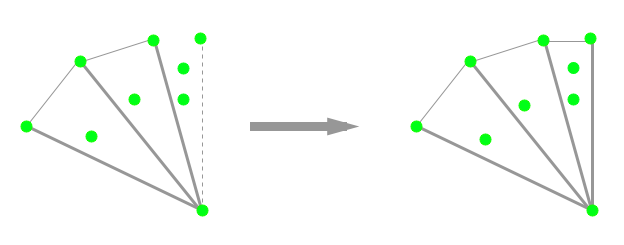
\includegraphics[scale=0.5]{img/ej31.png}

Como no hay nunca tres vértices alineados, toda tripla de vértices generará un triángulo válido.

Ahora bien, mientras se van agregando vértices hay que chequear que no se haya agregado un
triángulo que contenga enemigos. Además habrá que ver que el nuevo polígono es convexo y cuántos lugares
históricos fueron agregados de forma de mantener la información que se necesita para llegar a la solución final:

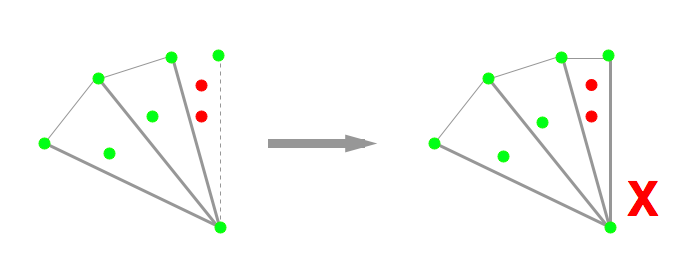
\includegraphics[scale=0.5]{img/ej32.png}

Como consecuencia de todo lo anterior, nuestro algoritmo precomputa desde el inicio para cada tripla de
vértices de puntos históricos distintos, la cantidad de puntos históricos y la cantidad de edificios enemigos dentro del
triángulo que generan (sin contarse a ellos mismos):

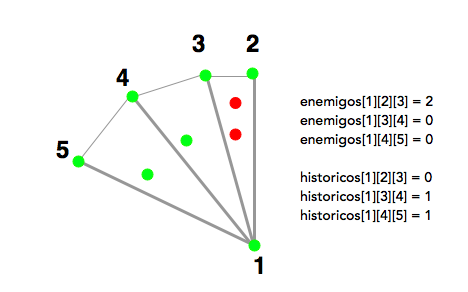
\includegraphics[scale=0.5]{img/ej33.png}

Teniendo toda esa información, vamos a querer armar para cada vértice $P$, un \textit{Convex Hull} a partir de $P$
si solo se consideran los vértices $V$ de puntos históricos que cumplan: $V.y > P.y \cup (V.y = P.y \cap V.x > P.x)$ con 
la cantidad máxima posible de lugares históricos y sin edificios enemigos. 
Es decir, solo contando los vértices que estén más arriba que $P$ o que tengan la misma coordenada $y$ pero estén más a
la derecha.

Esta restricción nos permite hacer un Graham Scan, ya que el algoritmo comienza tomando el punto más abajo y de
entre ellos el de más a la izquierda. Entonces si solo se consideran los puntos que cumplen la condición anterior,
se producirá un \textit{Convex Hull}. 

Notar que si probamos a todos los vértices posibles como el vértice de más abajo y más a la izquierda de entre ellos,
en algún momento el algoritmo va a considerar el vértice a partir del cual se forma el \textit{Convex Hull} buscado.

Sin embargo no es exactamente un Graham Scan lo que se va a hacer.

En primera instancia, ordenamos los vértices según el ángulo que forman con $P$ en sentido antihorario:

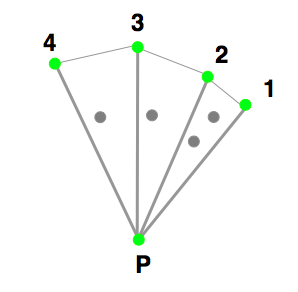
\includegraphics[scale=0.5]{img/ej34.png}

A medida que vamos armando el polígono convexo, hay que fijarse si se introducen edificios enemigos y cuántos
puntos históricos se van agregando. A su vez, como cualquier triángulo puede contener enemigos, no alcanza
con obtener un \textit{Convex Hull} para todos los puntos, sino que vamos a ir agregando triángulos gradualmente.

Como cada triángulo se determina mediante los dos puntos históricos diferentes a $P$, guardamos en un arreglo 
bidimensional $dp$ la máxima cantidad de puntos históricos que podemos tener sin contener enemigos en el polígono, si 
ese triángulo es el primero que agregamos (y solo agregamos triángulos en sentido horario). De esa manera, vamos 
chequeando si se pueden agregar vértices con un índice menor:

\centerline{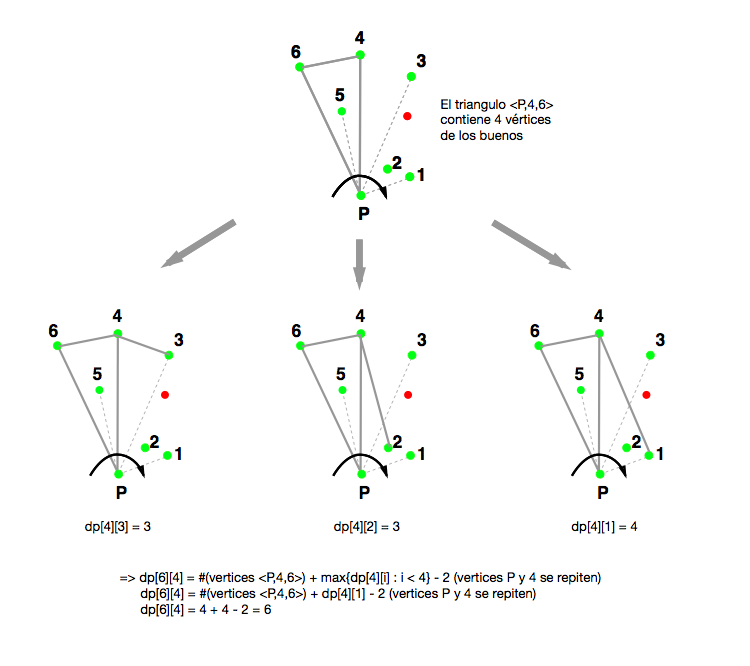
\includegraphics[scale=0.7]{img/ej35.png}}

Como vemos en la figura anterior, a partir de $i_1,...,i_n$ los puntos históricos que cumplen
$i_k.y > P.y \cup (i_k.y = P.y \cap i_k.x > P.x)$ ordenados en sentido antihorario según $P$, se definirán los
valores de $dp$. 

Sean $i_t, i_j \cap t > j$, si el primer triángulo que agrego es $<P,i_t,i_j>$ y los vértices que puedo agregar
para formar nuevos triángulos los agrego en sentido horario, tengo que buscar para cada $i_k \cap j > k$, cuántos
vértices podría agregarle al polígono si el primer triángulo que agrego es $<P,i_j,i_k>$, es decir $dp[j][k]$.
Si el triángulo $<P,i_t,i_j>$ contiene edificios enemigos, $dp[t][j] = 0$, en caso contrario:

\begin{equation*}
\begin{split}
    dp[t][j] & = \#\{ puntos\_historicos \in Triangulo(<P,i_t,i_j>)\} + 3 + \\
    & \max_{ i_k : j > k \cap valido(t,j,k) } \{dp[j][k]-2\} \\
    & = \#\{ k : k \in \{i_1,...,i_n\} \cap k \neq i \cap k \neq j \cap k \in Triangulo(<P,i_t,i_j>)\} + 3 + \\
    & \max_{ i_k : j > k \cap valido(t,j,k) } \{dp[j][k]-2\}
\end{split}
\end{equation*}

Donde $valido(t,j,k)$ es verdadero si y solo si el triángulo generado por $P, i_j, i_k$ no contiene edificios enemigos
y al unir el triángulo $P, i_t, i_j$ al $P, i_j, i_k$, el polígono sigue siendo convexo.

Notar que a $dp[j][k]$ se le resta 2 en la ecuación debido a que al unir el triángulo $P, i_t, i_j$ al $P, i_j, i_k$,
se están contando los puntos históricos $P, i_j$ dos veces.

\subsubsection{Pseudocódigo y correctitud}

En esta sección se detallarán las clases y los métodos importantes de la solución.

\subsubsection*{Clase punto}

Un Punto contendrá sus coordenadas $x,y$ ya que trabajamos sobre un espacio bidimencional. Asi mismo definimos
la igualdad de puntos por la igualdad de sus coordenadas. La suma y resta de puntos se define como la suma y resta
de sus coordenadas respectivamente. El producto crus $P \times Q = P_x * Q_y - Q_x * P_y$.

\subsubsection*{Clase segmento}

Un segmento contendrá simplemente un Punto origen $a$ y un Punto destino $b$. Asi se definen las funciones:

\begin{algorithm}[H]
	\caption{\textit{ContieneSegmentoPunto}}
	\Input{ Segmento $S$, Punto $P$ }
	\Output{ Bool }
	\Return{ValorAbsoluto((S.b-P) $\times$ (P-a)) $<$ epsilon \&\& \\
	min(S.a.x,S.b.x) - epsilon $\leq$ P.x \&\& P.x $\leq$ max(S.a.x, S.b.x) + epsilon \&\& \\
	min(S.a.y,S.b.y) - epsilon $\leq$ P.y \&\& P.y $\leq$ max(S.a.y, S.b.y) + epsilon}
\end{algorithm}

Es decir devuelve true si y solo si S.b-a y P-a son paralelos (y por lo tanto están en la misma recta infinita)
y además está dentro de los límites del segmento y no solo en la misma recta infinita.
Donde epsilon es una constante de valor positivo muy chico para prevenir errores de estabilidad numérica.

\begin{algorithm}[H]
	\caption{\textit{IntersecciónSegmentos}}
	\Input{ Segmento $S$, Segmento $Q$ }
	\Output{ Punto }
	Punto v1 = P.b - P.a \\
	Punto v2 = Q.b - Q.a \\
	bool paralelos = v1 $\times$ v2 == 0 \\
	\eIf{paralelos == false} {
		double alpha = (Q.a-a) $\times$ v2 / v1 $\times$ v2 \\
		Punto intersection = a + Punto(alpha * v1.x, alpha * v1.y)
		\If {S.ContieneSegmentoPunto(intersection) \&\& Q.ContieneSegmentoPunto(intersection))}{
			\Return{intersection}
		}
	}{
		\If {S.ContieneSegmentoPunto(Q.a))} {\Return{Q.a}}
		\If {S.ContieneSegmentoPunto(Q.b))} {\Return{Q.b}}
		\If {s.ContieneSegmentoPunto(a))} {\Return{a}}
		\If {s.ContieneSegmentoPunto(b))} {\Return{b}}
	}
	\Return{Null}
\end{algorithm}

Sabiendo que es más fácil hacer cuentas sobre rectas si tenemos la representación en formato $L(t)=a+t*(b-a)$ para
cada recta $L$ con puntos $a$ y $b$, obtenemos para ambos segmentos la resta $b-a$ y los guardamos en $v1$ y $v2$.
Lo que hace esta rutina es primero fijarse si las rectas son paralelas y como vimos en clase esto es verdadero
cuando $v1 \times v2$ es igual a 0. Si las rectas son paralelas, tienen intersección simplemente si alguna 
contiene un extremo de la otra. Si no son paralelas, también como vimos en clase, hay que buscar un alpha que
cumpla $alpha = (Q.a-a) \times v2 / v1 \times v2$ para encontrar la intersección entre las rectas si es que
fueran infinitas. Luego hay que fijarse si ambos segmentos contienen la intersección de las rectas infinitas
y si lo hacen, devolver la intersección.

\subsubsection*{Clase Triángulo}

Un triángulo se define mediante sus tres vértices extremos $a$, $b$ y $c$.
La operación importante para esta clase será:

\begin{algorithm}[H]
	\caption{\textit{ContieneTrianguloPunto}}
	\Input{ Triangulo $<a,b,c>>$, Punto $P$ }
	\Output{ Bool }
	double $leftmost\_x$ = min(a.x, min(b.x, c.x)) \\
	Segment $ray$ = Segment(Point($leftmost\_x$-1,p.y),p) \\
	int $intersections$ = 0 \\
	Segment $ab$ = Segment(a, b) \\
	Segment $bc$ = Segment(b, c) \\
	Segment $ca$ = Segment(c, a) \\
	\If {$ray$.InterseccionSegmentos($ab$) $\neq$ Null}{ $intersections$++ }
	\If {$ray$.InterseccionSegmentos($bc$) $\neq$ Null}{ $intersections$++ }
	\If {$ray$.InterseccionSegmentos($ca$) $\neq$ Null}{ $intersections$++ }
	\If {$ray$.ContieneSegmentoPunto(a))}{
		\If {b.y $<$ p.y}{ $intersections$ -= 1 }
		\If {c.y $<$ p.y}{ $intersections$ -= 1 }
	}
	\If {$ray$.ContieneSegmentoPunto(b))}{
		\If {a.y $<$ p.y}{ $intersections$ -= 1 }
		\If {c.y $<$ p.y}{ $intersections$ -= 1 }
	}
	\If {$ray$.ContieneSegmentoPunto(c))}{
		\If {a.y $<$ p.y}{ $intersections$ -= 1 }
		\If {b.y $<$ p.y}{ $intersections$ -= 1 }
	}
	\If {($ray$.ContieneSegmentoPunto(a) \&\& $ray$.ContieneSegmentoPunto(b)) $\|$ ($ray$.ContieneSegmentoPunto(a) \&\& $ray$.ContieneSegmentoPunto(c)) $\|$ ($ray$.ContieneSegmentoPunto(c) \&\& $ray$.ContieneSegmentoPunto(b))}{
		$intersections$ = 0
	}
	\Return{$intersections$ == 1 $\|$ $ab$.ContieneSegmentoPunto(p) $\|$ $bc$.ContieneSegmentoPunto(p) $\|$ $ca$.ContieneSegmentoPunto(p)}
\end{algorithm}

Lo primero que hacemos es calcular de los tres puntos del triángulo la menor coordenada $x$. A ese valor se
le resta 1 para asegurarse que se empieza desde un punto fuera del triángulo. Luego se crea un Segmento $ray$
horizontal desde $<leftmost\_x-1, p.y>$ hasta $P$. Como vimos en clase, el punto $P$ estará contenido en el 
triángulo si interseca con el mismo una cantidad impar de veces. Como no puede intersecarlo 3 veces, el punto
está adentro si hay exactamente una intersección con alguno de los segmentos $ab$, $bc$ o $ca$.
Luego hacemos un chequeo de casos borde. Puede pasar que $ray$ tenga una intersección con uno o dos vértices
del triángulo (tres no porque los tres vértices de un triángulo no pueden estar alineados). Como $ray$ es un
segmento horizontal, los casos posibles (según la coordenada $y$ de los tres puntos) son: 

\centerline{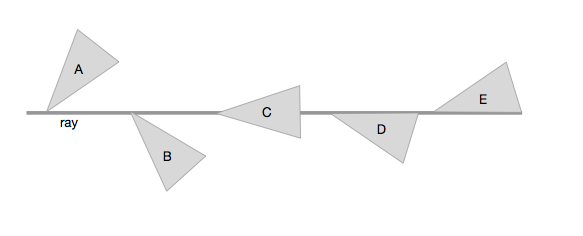
\includegraphics[scale=0.7]{img/ej36.png}}

Entonces lo que el algoritmo hace según los casos anteriores (entre los \textit{if} de las líneas 16-39) es:
\begin{itemize}
\item[A:] $intersections$ termina siendo 2 ya que se cuenta la misma dos veces, lo cual esta bien porque
no se quiere considerar que $ray$ entró en el triángulo.
\item[B:] $intersections$ termina siendo 0, lo cual esta bien porque
no se quiere considerar que $ray$ entró en el triángulo.
\item[C:] se cuenta el vértice como 1 intersección ya que se quiere considerar que $ray$ entró en el triángulo.
\item[D:] $intersections$ termina siendo 0 porque $ray$ interseca con dos vértices del triángulo, por lo
tanto la salida será true si y solo si el punto $P$ está adentro de uno de los bordes.
\item[E:] idem caso D.
\end{itemize}

Notar que todo lo anterior sirve si el punto no está incluido en alguno de los lados del triángulo, por este
motivo, si el punto esta contenido en los segmentos $ab, bc$ ó $ca$, devolvemos true (incluyendo el caso
en el que el punto sea uno de los vértices del triángulo).

\subsubsection*{Resolución del problema}

\begin{algorithm}[H]
	\caption{\textit{MaximosPuntosHistoricosEnMurallaConvexa}}
	\Input{ int $H$, int $E$, $vector<int>$ $historical\_places$, $vector<int>$ $enemy\_places$ }
	\Output{ int }

	$vector<vector<vector<int>>>$ $historical\_places\_in\_triangle$ = vector tridimencional de $H \times H \times H$ \\
	$vector<vector<vector<int>>>$ $enemy\_places\_in\_triangle$ = vector tridimencional de $H \times H \times H$

	\For {cada tripla de int $i,j,k$ diferentes entre 0 y $H-1$} {
        Punto $pi$ = $historical\_places$[i] \\
        Punto $pj$ = $historical\_places$[j] \\
        Punto $pk$ = $historical\_places$[k] \\
        \For {cada $l$ diferente a $i,j,k$ entre 0 y $H-1$} {
            Punto $pl$ = $historical\_places$[$l$] \\
            \If{Triangulo($pi,pj,pk$).ContienePuntoTriangulo(pl)}{
                $historical\_places\_in\_triangle$[i][j][k]++
            }
        }
        \For {int $l$ = 0 hasta $E-1$} {
            Punto $pl$ = $enemy\_places$[$l$] \\
            \If{Triangulo($pi,pj,pk$).ContienePuntoTriangulo(pl)}{
                $enemy\_places\_in\_triangle$[i][j][k]++
            }
        }
    }

	int $ans$ = min(2, $H$) \\
	\For{cada $i$ entre 0 y $H-1$}{
	    $ans$ = max($ans$, MaximosPuntosHistoricosDesde($i$, $H$, $E$, $historical\_places$, $enemy\_places$))
	}

	\Return{$ans$}
\end{algorithm}

Esta es la función principal del problema, tal como pide el enunciado recibe dos enteros $H,E$ con la cantidad
de puntos históricos y edificios enemigos y dos vectores $historical\_places$ y $enemy\_places$ con las coordenadas
de los mismos.
Con ellos, calcula y devuelve la máxima cantidad de puntos históricos que puede contener una
muralla convexa sin edificios enemigos dentro.

El algoritmo comienza declarando dos vectores tridimencionales $historical\_places\_in\_triangle$ y \\
$enemy\_places\_in\_triangle$ que contendrán para cada tripla de puntos diferentes, la cantidad de puntos históricos
y la cantidad de puntos enemigos dentro del triángulo que determina la tripla.
Luego el \textit{For} de las líneas 3-19 se encarga justamente de tomar triplas de tres puntos diferentes,
crear un triángulo y fijarse para cada punto histórico y edificio enemigo si está contenido en el triángulo, asi
calculando los valores de los dos vectores.

La línea 20 inicializa $ans$ como min(2, $H$) por el caso de que hayan menos de tres puntos hitóricos en la ciudad
y entonces se tenga que contruir una muralla para 0, 1 ó 2 puntos históricos (cosa que siempre es posible).

Finalmente el \textit{For} de las líneas 21-23 calcula para cada punto histórico, la respuesta al problema
si es que la muralla fuera armada a partir de ese punto uniéndolo mediante triángulos a otros puntos históricos
con coordenada $y$ mayor o coordenada $y$ equivalente y mayor coordenada $x$, todo esto tal como fue explicado
en la sección de \textbf{Explicación}. La respuesta es el máximo de estos valores, porque en algún momento el ciclo
toma el punto para el que se formará el \textit{Convex Hull} buscado (porque se prueba a partir de todos los puntos).

\bigskip

\begin{algorithm}[H]
	\caption{\textit{MaximosPuntosHistoricosDesde}}
	\Input{ int $ref\_point, $int $H$, int $E$, $vector<int>$ $historical\_places$, $vector<int>$ $enemy\_places$ }
	\Output{ int }
	Punto p = $historical\_places$[$ref\_point$] \\

    $vector<int>$ $valid\_historical\_places$ = \{ $i$ : $i$ entre 0 y $H-1$ y cumple que $historical\_places$[i] está más arriba que $p$ o tiene la misma coordenada $y$ pero mayor coordenada $x$ \} \\
    
    Ordenar $valid\_historical\_places$ según el ángulo de los puntos capturados con $P$ en sentido antihorario \\
    
    int V = $valid\_historical\_places$.size() \\
    $vector< vector<int> > dp$ = vector bidimencional relleno de 0 de tamaño $V \times V$ \\

    \For {cada $i$ de 0 a $V-1$} {
        int hi = $valid\_historical\_places$[i] \\
        \For {cada $j$ de 0 a $i-1$} {
            int hj = $valid\_historical\_places$[j] \\
            \If {$enemy\_places\_in\_triangle$[$ref\_point$][hi][hj] $\leq$ 0}{
	            int $h\_places$ = 3 + $historical\_places\_in\_triangle$[$ref\_point$][hi][hj] \\
	            $dp$[i][j] = $h\_places$ \\
	            \For {cada $k$ de 0 a $j-1$} {
	                int hk = $valid\_historical\_places$[k] \\
	                Punto r = $historical\_places$[hj] \\
	                Punto s = $historical\_places$[hi] \\
	                Punto q = $historical\_places$[hk] \\
	                bool $sigue\_convexo$ = (s-r) $\times$ (q-r) $>$ 0 \\
	                bool $sin\_enemigos$ = $enemy\_places\_in\_triangle$[$ref\_point$][hj][hk] == 0 \\
	                \If {$sigue\_convexo$ \&\& $sin\_enemigos$}{
						$dp$[i][j] = max($dp$[i][j], $h\_places$ + $dp$[j][k] - 2)
					}
	            }
            }
        }
    }

    \Return{$\max_{i,j}\{$dp$[i][j]\}$}
\end{algorithm}

Como fue explicado anteriormente, se quiere armar un \textit{Convex Hull} como si el punto con índice $ref\_point$
(que llamamos $P$) fuera el de más abajo y de entre ellos el de más a la izquierda.

Primero se filtran los puntos históricos que están arriba o tiene igual coordenada $y$ y mayor $x$ y se los guarda en 
el vector $valid\_historical\_places$.

Luego, de la misma manera que el Graham Scan se ordenan esos puntos según el ángulo que forman con $P$ (notar que no
hay dos con el mismo ángulo porque se garantiza que no hay tres vértices alineados). Esto se hace como en cualquier
algoritmo de ordenamiento pero definiendo el orden de manera que dos puntos $Q, R$ cumplen $Q < R$ si y solo si
$(Q-P) \times (R-P) > 0$. De esa manera ordenamos de menor a mayor para obtener los puntos en sentido antihorario.

Como paso siguiente, se crea el vector bidimencional $dp$ que para $i > j$, $dp[i][j]$ contiene la máxima cantidad de 
puntos históricos que podemos tener en el polígono convexo triangulado sin contener enemigos, si
ese triángulo es el primero que agregamos (y solo agregamos triángulos en sentido horario).

De esa manera, y como fue explicado antes, entre las líneas 6-26 rellenamos $dp$ tal que, sean 
$hvi = historical\_places[valid\_historical\_places[i]]$ y $hvj = historical\_places[valid\_historical\_places[j]]$:
\begin{equation*}
\begin{split}
    dp[i][j] & = \#\{ puntos\;historicos \in Triangulo(<P, hvi, hvj>)\} + 3 + \\
    & \max_{ k : j > k \cap valido(i,j,k) } \{dp[j][k]-2\}
\end{split}
\end{equation*}

Donde $valido(t,j,k)$ es verdadero si y solo si:
\begin{itemize}
\item Sean $hvi = historical\_places[valid\_historical\_places[i]]$, $hvj = historical\_places[valid\_historical\_places[j]]$ y
$hvk = historical\_places[valid\_historical\_places[k]]$.
\item El triángulo generado por $<P, hvj, hvk>$ no contiene edificios enemigos cosa que se chequea en la línea 19.
\item Al unir el triángulo $<P, hvi, hvj>$ al $<P, hvj, hvk>$, el polígono sigue siendo convexo (lo cual comprobamos en la línea 18).
\end{itemize}

Finalmente devolvemos $\max_{i,j}\{dp[i][j]\}$, es decir, la cantidad de puntos históricos del \textit{Convex Hull} a partir de $P$
sin enemigos que contiene la máxima cantidad de puntos históricos.

\subsubsection{Complejidad}

Los algoritmos de las clases Punto, Segmento y Triángulo tienen todos complejidad $O(1)$ ya que solo hacen asignaciones y
comparaciones y la cantidad de operaciones es siempre fija.

El algoritmo MaximosPuntosHistoricosDesde:

\begin{itemize}
\item Declara un punto $P$, un vector $valid\_historical\_places$ filtrando $historical\_places$ (de tamaño $H$),
un int $V$, un vector bidimencional $dp$ de tamaño $V \times V$ y ordena $valid\_historical\_places$. Como $V$ es el tamaño
del vector resultante de filtrar $historical\_places$, $V \leq H$.
Entonces todo esto tiene una complejidad de $O(1+H+V+V*+H*log(H)) = H*log(H)$
\item Para cada $i$ entre 0 y $H-1$ y para cada $j$ entre 0 y $i-1$: declara los ints $hi$ y $hj$, se fija el valor de \\
$enemy\_places\_in\_triangle[ref\_point][hi][hj]$ y hace dos asignaciones en $h\_places$ y $dp[i][j]$. Además para cada
$k$ entre 0 y $j-1$ entre las líneas 11 y 22 hace varias comparaciones y asignaciones, pero todas de complejidad constante.
Todo esto tiene una complejidad de $O(H*(1+H*(1+H*1))) = O(H^3)$
\item Busca el máximo de $dp$, que es un vector bidimencional de $V \times V$. Complejidad $O(V^2) = O(H^2)$
\end{itemize}

Entonces sumando todo MaximosPuntosHistoricosDesde es $O(H*log(H)+H^3+H^2) = O(H^3)$.

Finalmente, el algoritmo principal, MaximosPuntosHistoricosEnMurallaConvexa:

\begin{itemize}
\item Declara dos vectores tridimecionales de tamaño $H \times H \times H$. Complejidad $O(H^3)$
\item Para cada $i,j,k$ diferentes entre 0 y $H-1$: declara tres puntos $pi,pj,pk$, para cada $l$ entre 0 y $H-1$
realiza comparaciones y asignaciones constantes entre las líneas 8-11 y para cada $l$ entre 0 y $E-1$
realiza comparaciones y asignaciones constantes entre las líneas 14-17. Complejidad $O(H^3*(1+H+E)) = O(H^3*(H+E))$
\item Declara un int $ans$ y para cada $i$ entre 0 y $H-1$ hace un llamado a la función MaximosPuntosHistoricosDesde que como
se vio anteriormente es $O(H^3)$. Entonces esto tiene complejidad $O(H^4)$.
\end{itemize}

Teniendo en cuenta que $N = H+E$ y entonces $H \leq N$ y $E \leq N$, la complejidad total de MaximosPuntosHistoricosEnMurallaConvexa
es: $O(H^3+H^3*(H+E)+H^4) = O(N^3+N^4+N^4) = O(N^4)$.

\subsection{Casos de test}

\subsubsection*{Caso 1}

\begin{center}
    \begin{tabular}{| l | l |}
    \hline
    Entrada & Salida \\ \hline
	6 3 & 5 \\
	0 0 & \\
	1 4 & \\
	4 5 & \\
	6 5 & \\
	9 4 & \\
	10 0 & \\
	4 1 & \\
	6 1 & \\
	8 3 & \\
	\hline
    \end{tabular}
\end{center}

Gráficamente:

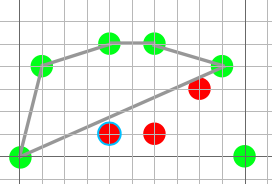
\includegraphics[scale=0.5]{img/ej3c1.png}

\subsubsection*{Caso 2}

\begin{center}
    \begin{tabular}{| l | l |}
    \hline
    Entrada & Salida \\ \hline
	7 0 & 7 \\
	0 0 & \\
	1 5 & \\
	2 4 & \\
	3 1 & \\
	4 0 & \\
	5 2 & \\
	5 3 & \\
	\hline
    \end{tabular}
\end{center}

Gráficamente:

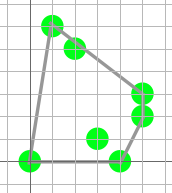
\includegraphics[scale=0.5]{img/ej3c2.png}

\subsubsection*{Caso 3}

\begin{center}
    \begin{tabular}{| l | l |}
    \hline
    Entrada & Salida \\ \hline
	4 2 & 2 \\
	0 0 & \\
	1 0 & \\
	-1 3 & \\
	2 3 & \\
	0 1 & \\
	1 1 & \\
	\hline
    \end{tabular}
\end{center}

Gráficamente:

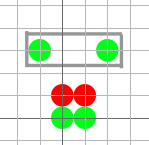
\includegraphics[scale=0.5]{img/ej3c3.png}

\subsubsection*{Caso 4}

\begin{center}
    \begin{tabular}{| l | l |}
    \hline
    Entrada & Salida \\ \hline
	10 6 & 6 \\
	0 0 & \\
	0 6 & \\
	2 9 & \\
	-2 9 & \\
	4 8 & \\
	-4 8 & \\
	5 5 & \\
	-5 5 & \\
	6 1 & \\
	-6 1 & \\
	3 1 & \\
	-3 1 & \\
	3 4 & \\
	-3 4 & \\
	4 7 & \\
	-4 7 & \\
	\hline
    \end{tabular}
\end{center}

Gráficamente:

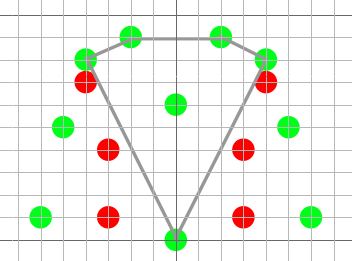
\includegraphics[scale=0.5]{img/ej3c4.png}

\newpage
\section{Ejercicio 4}

Peso asignado: 6.

\subsection{Introducción}

En este problema se pedía un algoritmo que dada una permutación $P$ de números
entre 1 y $N$, devolviera la cantidad de grafos torneos de $N$ nodos que fueran
isomorfos a sí mismos luego de haber aplicado $P$ sobre el conjunto de vértices.
Dado que el resultado podía llegar a tomar valores muy grandes la respuesta
se devuelve módulo $10^9 + 7$. Por último, la complejidad temporal pedida era
$\ord(N^2 \times \log N)$ pudiendo esta ser mejorada a $\ord(N \times \log N)$.

\subsection{Solución}

\subsubsection{Permutación como conjunto de ciclos}

La solución propuesta utiliza fuertemente el hecho de que una permutación $P$ de
números entre 1 y $N$ puede ser representada mediante un conjunto de ciclos
dirigidos donde cada arco $(u, v)$ corresponde a $(u, P(u))$ donde $P(u) = v$.

\newcolumntype{M}[1]{>{\centering\arraybackslash}m{#1}}

\begin{table}[H]
    \caption{Ejemplo de permutación $P$ con $N = 4$.} \label{ej4:table:perm}
    \centering
    \begin{tabular}{|c|M{2em}|M{2em}|M{2em}|M{2em}|}
        \hline
        $x$ & 1 & 2 & 3 & 4 \\
        \hline
        $P(x)$ & 2 & 3 & 1 & 4 \\
        \hline
    \end{tabular}
\end{table}

\begin{figure}[H]
    \caption{Representación de la permutación definida en el Cuadro
    \ref{ej4:table:perm} mediante ciclos dirigidos.} \label{ej4:fig:perm}
    \centering
    \begin{tikzpicture}
        \SetGraphUnit{2}
        \GraphInit[vstyle=Normal]
        \tikzset{EdgeStyle/.style={->}}
        \Vertex{1}
        \EA(1){2}
        \SO(1){3}
        \EA(3){4}
        \Edge[style={bend left=30}](1)(2)
        \Edge[style={bend left=30}](2)(3)
        \Edge[style={bend left=30}](3)(1)
        \Loop[dist=4em,dir=SOEA](4)
    \end{tikzpicture}
\end{figure}

A raíz de esto lo primero que haremos será estudiar las permutaciones formadas
por únicamente un ciclo.

\subsubsection{Permutaciones de un ciclo} \label{ej4:sec:unciclo}

Lo que interesa analizar es el número de grafos torneos de tamaño $N$ que luego
de aplicarles la permutación $P$ son isomorfos al grafo torneo original. Un
grafo torneo es un grafo completo donde todas las aristas tienen asignada una
dirección. Formalmente, se desea contar los grafos torneo $G$ que cumplen
$(\forall (v, w) \in E(G)) (P(v), P(w)) \in E(P(G))$.

Una condición necesaria para que se cumpla esto, es que todos los elementos
pertenecientes al mismo ciclo de una permutación posean el mismo grado de
entrada y salida entre sí en el grafo torneo.

Supongamos que esto no es cierto, entonces debería existir un par de vértices
$v_0, w_0 (v_0 \neq w_0)$ con distinto grado de salida pertenecientes a un grafo
torneo isomorfo a su permutación de un ciclo. Tanto $v_0$ y $w_0$ tendrán un
predecesor en la permutación vista como ciclo. Llamemos $v_1$ el vértice tal que
$P(v_1) = v_0$ y $w_1$ el que cumple $P(w_1) = w_0$. Para que $G$ sea isomorfo a
su permutación, como $v_1$ toma el lugar de $v_0$, tiene que tener el mismo
grado de salida, lo mismo con $w_1$ y $w_0$. Este razonamiento se puede aplicar
a los predecesores de $v_1$ y $w_1$, forzando a que existan $v_2$ y $w_2$
manteniendo los correspondientes grados de salida. Si se sigue aplicando esta
lógica, llegará un momento donde el predecesor de $v_k$ será $w_0$ o bien el de
$w_k$ será $v_0$. Esto implica que $P(w_0) = v_k$ o $P(v_0) = w_k$, lo cual no
es posible, ya que teniendo distinto grado de salida el isomorfismo no sería
valido. La demostración es análoga para el grado de entrada.

Habiendo dicho esto, demostraremos que para permutaciones que forman un ciclo
par, no existe un grafo torneo que sea isomorfo al aplicarle la misma. Si el
ciclo es par, el grafo torneo correspondiente tiene un número par de nodos.
Supongamos que es posible asignarle el mismo grado de salida a todos los nodos,
para ello podemos utilizar la siguiente igualdad: $\sum_{v \in V(G)} d_{out}(v)
= \#E(G)$. Asumamos que el grado de salida es $k$ para todos los vértices,
entonces tenemos: $N \times k = \#E(G) = \frac{N \times (N - 1)}{2}$. Dividiendo
por $N$ de ambos lados nos queda $k = \frac{N - 1}{2}$ que como $N$ es par, $N -
1$ es impar, por lo tanto no divisible por 2. Queda así demostrado que si el
tamaño del ciclo de la permutación es par, no es posible asignarles el mismo
grado a todos los nodos lo cual lleva a que no se cumpla la condición necesaria
enunciada anteriormente.

Para los ciclos impares primero veremos que es posible tener todos los nodos con
el mismo grado de salida, luego demostraremos la cantidad de grafos torneos que
cumplen lo pedido en función del tamaño del ciclo.

Aplicando la misma igualdad que en el párrafo anterior tenemos $N \times k =
\#E(G) = \frac{N \times (N - 1)}{2}$ donde al dividir por $N$ de ambos lados nos
queda $k = \frac{N - 1}{2}$ que ahora teniendo $N$ impar, $N - 1$ es par, por lo
tanto divisible por 2. Así llegamos a que no sólo es posible asignarle el mismo
grado de salida a cada nodo si no que además el mismo vale $\frac{N - 1}{2}$.

Queda entonces ver cuántos grafos torneo cumplen ser isomorfos con su
permutación siendo esta un ciclo impar. Para esto se utilizará un argumento
similar al utilizado para probar que no podían existir dos vértices con distinto
grado. Sabemos que todos los nodos tienen $\frac{N - 1}{2}$ arcos salientes y
por ende $\frac{N - 1}{2}$ arcos entrantes, lo que habría que demostrar es cómo
asignarlos en cada vértice de forma tal que se cumpla el isomorfismo.

A continuación demostraremos que únicamente los grafos torneos donde todos los
vértices se conectan de la misma forma hacia sus $\frac{N - 1}{2}$ sucesores del
ciclo de la permutación forman un isomorfismo válido. Supongamos que esto no es
cierto, por lo tanto existe un par de vértices $v_0, w_0 (v_0 \neq w_0)$ que se
conecta de forma distinta a los correspondientes $\frac{N - 1}{2}$ sucesores del
ciclo de la permutación. Aquí es donde aplicamos el mismo razonamiento que en la
demostración de los grados de los vértices. Existen $v_1$ y $w_1$ tal que
$P(v_1) = v_0$ y $P(w_1) = w_0$ los cuales al tomar el lugar de $v_0$ y $w_0$ en
el grafo torneo permutado deberán estar conectados de la misma forma a sus
$\frac{N - 1}{2}$ sucesores. Se realiza el proceso de ir repitiendo este
razonamiento en los predecesores hasta que se tiene $P(v_0) = w_k$ o $P(w_0) =
v_k$ que como difieren en la forma de saltar a sus sucesores no permite un
isomorfismo válido.

Habiendo probado esto, calcular el número de grafos torneo posibles para una
permutación correspondiente a un ciclo impar de longitud $N$ es equivalente a
contar la cantidad de formas en las que un vértice puede saltar a sus $\frac{N -
1}{2}$ sucesores. Cada arco puede ser tanto saliente como entrante, y se tienen $\frac{N -
1}{2}$ a definir, por lo tanto un total de $2^{\frac{N -1}{2}}$ combinaciones
posibles.

\subsubsection{Permutaciones entre ciclos} \label{ej4:sec:paresciclos}

Como se ve en la Figura \ref{ej4:fig:perm}, una permutación puede estar
representada por más de un ciclo. Vimos cómo calcular el número de combinaciones
que brinda un ciclo en particular ahora es necesario ver las combinaciones
posibles entre todos los que componen la permutación.

Para esto estudiaremos las combinaciones posibles entre un par de ciclos, ya que
veremos las combinaciones que suman los otros ciclos son independientes entre
sí. Teniendo dos ciclos impares $C_0$ y $C_1$ para obtener un grafo torneo deben
existir todas las aristas entre ellos con una dirección asignada.

El número de aristas a asignar en total corresponde a $|C_0| \times |C_1|$.
Cuando se agrega una arista entre ciclos, inmediatamente se está definiendo la
dirección de otras aristas entre ambos. Esto es consecuencia del mismo proceso
estudiado para calcular el número de permutaciones dentro de un mismo ciclo. Al
agregar una arista $(u, v)$ donde $u \in C_0$ y $v \in C_1$, para que la
permutación resulte en el mismo grafo torneo, también debe existir $(P(u),
P(v))$. Esto se repite hasta que para algún par $(u', v')$ se tenga que $(P(u'),
P(v')) = (u, v)$. La pregunta entonces es cuántas aristas son asignadas hasta
llegar al punto donde se vuelve a la primera. Cada arista agregada avanza en uno la
posición de ambos ciclos de permutaciones, por lo tanto, el número de aristas
que se deben agregar para que ambos ciclos vuelvan a la posición inicial
corresponde al mínimo común múltiplo entre $|C_0|$ y $|C_1|$. Finalmente,
teniendo el total de aristas a agregar y la cantidad que se agregan como
consecuencia de una arista nueva podemos calcular cuántos grupos de aristas
habrán. Tomando el número total de aristas a agregar y dividiéndolo por el mínimo común
múltiplo se obtiene $\frac{|C_0| \times |C_1|}{MCM(|C_0|, |C_1|)}$ que
corresponde con el valor del máximo común divisor $MCD(|C_0|, |C_1|)$.

Lo último a notar es que cada grupo de aristas que se agrega puede tener
asignada una dirección distinta a la de los grupos anteriores. Por lo tanto, la
cantidad de formas de orientar las aristas entre dos ciclos corresponde a
$2^{MCD(|C_0|, |C_1|)}$.

El hecho de que cada par de ciclos agregue independientemente del resto esta
cantidad de combinaciones posibles se debe a que la forma en la que un ciclo
asigna sus arcos para sí mismo así como contra el resto de los ciclos no afecta
la elección de arcos contra el par elegido en particular. Lo único que se asume
es que se comienza con dos ciclos impares cuya asignación de arcos para sí y
contra el resto es válida con respecto al isomorfismo buscado.

\subsubsection{Algoritmo \emph{Divide \& Conquer}}

El algoritmo desarrollado para contar el total de combinaciones posibles hace
uso de la técnica algorítmica \emph{Divide \& Conquer} donde dado un arreglo $C$ con
los tamaños de los ciclos correspondientes a la permutación realiza los
siguientes pasos:

\begin{itemize}
	\item Si $|C| = 1$, si el tamaño del ciclo es par, devuelvo 0, caso contrario
    $2^{\frac{N -1}{2}}$ con $N$ siendo el tamaño del ciclo.
    \item Si $|C| > 1$ entonces llamo el algoritmo sobre el intervalo $\left[0,
    \frac{|C|}{2} \right)$ y $\left[\frac{|C|}{2}, |C| \right)$, multiplico
    ambos resultados y los multiplico a su vez por el número de combinaciones
    entre los ciclos de ambas mitades.
\end{itemize}

A continuación se presenta el pseudocódigo del algoritmo que aplica \emph{Divide
\& Conquer}:

\begin{algorithm}[H]
    \caption{Número de grafos torneos isomorfos a su permutación $P$}
    \Input{Arreglo $C$ con las longitudes de los ciclos de $P$ e índices $i$ y
    $j$,}
    \Output{Devuelve el número de grafos torneos isomorfos a sí mismos con la
    permutación $P$ módulo $10^9 + 7$.}

    \eIf{$j - i == 0$} {
        \Return{1} \;
    }
    {
        \eIf{$j - i == 1$} {
            \Return{\emph{$0$ si el ciclo es impar, $2^{\frac{C[i] - 1}{2}}$ caso
            contrario}} \;
        }
        {
            \emph{primeraMitad} $\gets$
                \emph{calcular y guardar combinaciones posibles para los ciclos
                en el intervalo $\left[ i, \frac{i + j}{2} \right)$} \;
            \emph{segundaMitad} $\gets$
                \emph{calcular y guardar combinaciones posibles para los ciclos
                en el intervalo $\left[ \frac{i + j}{2}, j \right)$} \;
            \emph{combinacionesPosibles} $\gets$
                \emph{(primeraMitad $\times$ segundaMitad)
                \% $(10^9 + 7)$} \;
            \emph{combinacionesPosibles} $\gets$
                \emph{(combinacionesPosibles $\times$
                número de combinaciones entre ciclos de ambas mitades)
                \% $(10^9 + 7)$} \;

            \Return{\emph{combinacionesPosibles}} \;
        }
    }
\end{algorithm}

El algoritmo anterior recibe como entrada un arreglo $C$ con las longitudes de
los ciclos de $P$, el mismo se genera mediante el siguiente algoritmo:

\begin{algorithm}[H]
    \caption{Longitudes de ciclos de permutación $P$}
    \Input{Arreglo con la permutación $P$.}
    \Output{Devuelve un arreglo $C$ con las longitudes de los ciclos de la
    permutación $P$.}

    \emph{longitudesCiclos} $\gets$ \emph{lista vacía} \;
	\For{\emph{i} \textbf{en} $\left[ 0, |P| \right)$} {
        \If{\emph{$P[i]$ no fue visitado}} {
            \emph{longitudCiclo} $\gets$ $1$ \;
            \emph{j} $\gets$ \emph{i} \;
            \emph{marcar a $P[j]$ como visitado} \;
            \While{$P[j] \neq j + 1$} {
                \emph{longitudCiclo} $\gets$ \emph{longitudCiclo} + 1 \;
                \emph{j} $\gets$ $P[j]$ \;
                \emph{marcar a $P[j]$ como visitado} \;
            }
            \emph{longitudesCiclos}\textbf{.agregar}(\emph{longitudCiclo}) \;
        }
    }
    \Return{\emph{longitudesCiclos}} \;
\end{algorithm}

Por último, el algoritmo utilizado para calcular las combinaciones entre ciclos
de dos mitades:

\begin{algorithm}[H]
    \caption{Cantidad de combinaciones entre los ciclos de la primer y segunda
    mitad}
    \Input{Arreglo $C$ con longitudes de ciclos e índices $i$ y $j$.}
    \Output{Cantidad de combinaciones posibles entre los ciclos de la primera y
    la segunda mitad.}

    \emph{totalPermutaciones} $\gets$ 1 \;
    \emph{ciclosPrimeraMitad} $\gets$ \emph{diccionario donde las llaves son los
    tamaños de los ciclos y los valores la cantidad existente con ese tamaño
    para la primer mitad} \;
    \emph{ciclosSegundaMitad} $\gets$ \emph{diccionario donde las llaves son los
    tamaños de los ciclos y los valores la cantidad existente con ese tamaño
    para la segunda mitad} \;

    \ForEach{\emph{clavePrimeraMitad} \textbf{en} \emph{ciclosPrimeraMitad}} {
        \ForEach{\emph{claveSegundaMitad} \textbf{en} \emph{ciclosSegundaMitad}} {
            \emph{máximoComúnDivisor} $\gets$
                \emph{máximo común divisor entre clavePrimeraMitad y claveSegundaMitad} \;
            \emph{permutaciones} $\gets$
                $(2^{\emph{máximoComúnDivisor}})^{\emph{ciclosSegundaMitad[claveSegundaMitad]}}$ \;
            \emph{permutaciones} $\gets$
            $\emph{permutaciones}^{ciclosPrimeraMitad[clavePrimeraMitad]}$ \;
            \emph{totalPermutaciones} $\gets$
            \emph{totalPermutaciones} $\times$ \emph{permutaciones}
            \emph{\% $(10^9 + 7)$} \;
        }
    }
    \Return{\emph{totalPermutaciones}} \;
\end{algorithm}

\subsubsection{Correctitud}

Para ver que el algoritmo es correcto es posible realizar inducción sobre el
tamaño del arreglo $C$ con las longitudes de ciclos de la permutación $P$. El
caso base sería arreglo de un elemento donde vemos que es correcto ya que hace
la cuenta desarrollada en la Sección \ref{ej4:sec:unciclo} para calcular el
número de combinaciones con un único ciclo. Para el paso inductivo, teniendo
como hipótesis inductiva que el algoritmo funciona para arreglos $C$ de longitud
$N - 1$ es posible asumir que las llamadas a las dos mitades calculan de forma
correcta las combinaciones posibles en cada una de ellas. Por lo tanto, una vez
que se calculan todas las posibles combinaciones entre ellas siguiendo lo
descrito en la Sección \ref{ej4:sec:paresciclos} el algoritmo es correcto para
$N$.

\subsection{Complejidad teórica}

El algoritmo desarrollado tiene una complejidad temporal $\ord(N \times \log
N)$. Para probar esto estudiaremos la resolución de a partes.

Lo primero que se hace es transformar la permutación $P$ en el arreglo con
longitudes de ciclos $C$. Esto tiene un costo $\ord(N)$ ya que se iteran los
elementos de $P$ y al marcarlos como visitados no se vuelven a recorrer los
ciclos que ya se agregaron.

Para demostrar la complejidad del \emph{Divide \& Conquer} primero estudiaremos
la complejidad de calcular las combinaciones posibles entre dos mitades de
ciclos.

En esta rutina primero se cuenta la cantidad de ciclos de cierta
longitud que hay en cada mitad. Esto en el peor caso es $\ord(N)$, que sería
cuando todos los ciclos son de un único elemento. A esto se le suma el recorrer
ambos mapas y generar el producto correspondientes. Cada mapa tiene a lo sumo
tamaño $\sqrt{N}$ ya que si hubiera más de $\sqrt{N}$ tamaños de ciclos entonces
la suma de los mismos sería distinta a $N$. Por lo tanto, la iteración de ambos
mapas tiene un costo $\ord(\sqrt{N} \times \sqrt{N}) = \ord(N)$. El costo de
calcular las potencias módulo $10^9 + 7$ es constante puesto que siempre se está
operando con valores módulo $10^9 + 7$, por lo tanto la operación es sobre una
entrada que está acotado por una constante.

Así demostramos entonces que calcular las combinaciones entre ambas mitades
tiene costo lineal. Luego, dado que el \emph{Divide \& Conquer} parte a
la mitad hasta llegar a elementos de tamaño uno, el mismo llama $\ord(\log{N})$
veces el paso de \emph{merge} donde se realiza la llamada con costo lineal más
los productos que ya dijimos eran constantes.

Por lo tanto, tenemos $\ord(N \times \log N)$ como complejidad temporal.

\subsection{Casos de prueba}

Para probar el correcto funcionamiento del algoritmo se realizaron pruebas a
distinto nivel:

\begin{itemize}
    \item Pruebas sobre la función de potencia con módulo
    \item Pruebas sobre la función que cuenta los ciclos en $P$
    \item Pruebas sobre la función que cuenta la cantidad de combinaciones entre
    dos mitades de ciclos
    \item Pruebas sobre la función que cuenta el total de torneos isomorfos a su
    permutación $P$
\end{itemize}

Los primeros tres tipos de pruebas fueron para asegurar el correcto
funcionamiento con números que estuvieran por debajo y encima del valor $10^9 +
7$, así como ver que cada módulo cumpliera correctamente su función para
distintos tipos de permutaciones (de un único ciclos, varios ciclos, ciclos
formados por un único elemento).

La última prueba verifica la funcionalidad final del algoritmo, utilizando primero
entradas pequeñas controladas con distintos tipos de permutaciones:

\begin{itemize}
    \item Un ciclo de un elemento
    \item Un ciclo de tres elementos
    \item Dos ciclos
    \item Tres ciclos
    \item Cuatro ciclos de un elemento
    \item Ciclos pares
\end{itemize}

Y por último buscando probar resultados que excedieran el valor $10^9 +
7$ por un lado, y por el otro con permutaciones de tamaño $10^5$ para corroborar
que el algoritmo pudiera manejar ese tamaño de entrada.


\end{document}
